%
% File graph_system.tex
%

\documentclass[11pt,a4paper]{article}
\usepackage[hyperref]{acl2017}
\usepackage{times}
\usepackage{url}
\usepackage{latexsym}
\usepackage{amsmath}
\usepackage{breqn}
\usepackage{pgfplotstable}
\usepackage{algorithm2e}
\usepackage{hhline}
\usepackage{multirow}
\usepackage[font=small]{caption}
\usepackage{subcaption}
\usepackage{color}
\usepackage{float}
\usepackage{lipsum,adjustbox}
\usepackage{tikz}
\usepackage{tikz-dependency}
\usepackage{enumitem}
\usepackage{xr}
\externaldocument{acl2017_supp}
\usetikzlibrary{shapes,fit,calc,er,positioning,intersections,decorations.shapes,mindmap,trees}
\tikzset{decorate sep/.style 2 args={decorate,decoration={shape backgrounds,shape=circle,
      shape size=#1,shape sep=#2}}}
\newcommand{\oa}[1]{\footnote{\color{red} #1}}
\newcommand{\daniel}[1]{\footnote{\color{blue} #1}}
\newcommand{\com}[1]{}
\newcommand{\parser}[1]{TUPA\textsubscript{#1}}
\newcommand{\secref}[1]{Section~\ref{#1}}
\newcommand{\figref}[1]{Figure~\ref{#1}}
\newcommand{\tabref}[1]{Table~\ref{#1}}
\DeclareMathOperator*{\argmin}{argmin}
\DeclareMathOperator*{\argmax}{argmax}
\SetKwRepeat{Do}{do}{while}

\def\linkspace#1#2{\leavevmode
\def\tmp##1{\nolinebreak[2]\href{#1}{\hbox{##1}}}%
\xlinkspace#2 \relax}

\def\xlinkspace#1 #2{%
 \ifx\relax#2%
 \xlinkdash#1-\relax
 \else
 \xlinkdash#1 -\relax
 \expandafter\xlinkspace\expandafter#2%
 \fi}

\def\xlinkdash#1-#2{%
 \ifx\relax#2%
 \tmp{#1}%
 \else
 \tmp{#1-}%
 \expandafter\xlinkdash\expandafter#2%
 \fi}

%\aclfinalcopy % Uncomment this line for the final submission
\def\aclpaperid{***} %  Enter the acl Paper ID here

%\setlength\titlebox{5cm}
% You can expand the titlebox if you need extra space
% to show all the authors. Please do not make the titlebox
% smaller than 5cm (the original size); we will check this
% in the camera-ready version and ask you to change it back.

\title{A Complete and Sound Transition System for Graph Parsing}

\author{Daniel Hershcovich$^{1,2}$ \\
  $^1$The Edmond and Lily Safra Center for Brain Sciences \\
  $^2$School of Computer Science and Engineering \\
  Hebrew University of Jerusalem \\
  \texttt{danielh@cs.huji.ac.il}
}

\date{}

\begin{document}
\maketitle

%%%%%%%%%%%%%%%%%%%%%%%%%%%%%%%%%%%%%%%%%%%%%%%%%%%%%%%%%%%%%%%
%%%%%%%%%%%%%%%%%     Abstract     %%%%%%%%%%%%%%%%%%%%%%%%%%%%
%%%%%%%%%%%%%%%%%%%%%%%%%%%%%%%%%%%%%%%%%%%%%%%%%%%%%%%%%%%%%%%
\begin{abstract}
Transition systems have been proposed for many tasks in NLP.
We present a general transition system that is complete and sound with respect to graph parsing,
and verify experimentally that it is suitable for many different representation schemes.
\end{abstract}


%%%%%%%%%%%%%%%%%%%%%%%%%%%%%%%%%%%%%%%%%%%%%%%%%%%%%%%%%%%%%%%
\section{Introduction}\label{sec:introduction}

Transition-based parsing is a widely used framework for natural language parsing.
Transition-based parsers scan the text from start to end,
and create the parse incrementally by applying a \textit{transition}
at each step to the parser's state,
defined using three data structures: a buffer $B$ of tokens and nodes to be processed,
a stack $S$ of nodes currently being processed,
and a graph $G=(V,E,\ell)$ of constructed nodes and edges,
where $V$ is the set of \emph{nodes}, $E$ is the set of \emph{edges},
and $\ell : E \to L$ is the \emph{label} function, $L$ being the set of possible labels.
Some states are marked as \textit{terminal}, meaning that $G$ is the final output.
A classifier is used at each step to select the next transition based on features
encoding the parser's current state.
During training, an oracle creates training instances for the classifier,
based on gold-standard annotations.

Many variations to this model have been proposed, such as using more than one stack to support
non-projective dependency parsing \cite{gomez2010a},
as well as easy-first parsing rather than following the order of tokens \cite{goldberg2010efficient}.

A \textit{transition system} \cite{Nivr:06,nivre2008algorithms} may in general be used to cast structure prediction
problems as sequence prediction problems.
The framework has been applied successfully to many NLP tasks
\cite[][among others]{bohnet2012transition,lample-EtAl:2016:N16-1,kiperwasser2016simple,zhang-zhang-fu:2016:P16-1,kong2017dragnn,hershcovich2017a,zhou2017neural}.

\paragraph{Anchored graphs.}
We introduce the notion of an \textit{anchored graph},
a generalization of existing notions such as (semantic) dependency graph and phrase structure graph,
as well as UCCA DAGs and AMRs.
An anchored graph $G$ over a sequence $\langle w\rangle_1^n=w_1, \ldots, w_n$ of tokens
(or \textit{terminals}) is a labeled graph $G=(V,E)$ where $\langle w\rangle_1^n \subseteq V$ and
$\mathrm{deg}^+(w_i) = 0$ for all $i=1,\ldots,n$ (the terminals have no outgoing edges).
Since parsing of natural language is inherently based on the uttered tokens,
we claim this formulation is general enough to encompass all parsing schemes.

Broad coverage of graph structures is important for parsing of current semantic representation schemes
\cite{abend2017state}, which exhibit structural properties traditionally ignored in transition-based
parsing.
One such property is \textit{reentrancy},
namely the sharing of semantic units between predicates.
For instance, in \figref{fig:graduation},
``John'' is an argument of both ``graduation''
and ``moved'', yielding a graph rather than a tree.
A second property is \textit{discontinuity},
as in \figref{fig:gave}, where ``gave up'' forms a discontinuous semantic unit.
Discontinuities are pervasive, e.g.,  with multi-word
expressions \cite{schneider2014discriminative}.
Finally, unlike most dependency schemes, some schemes (e.g. UCCA, AMR) use \textit{non-terminal nodes}
to represent units comprising more than one word.
The use of non-terminal nodes is motivated by constructions with no clear head, including
coordination structures (e.g., ``John and Mary'' in \figref{fig:home}),
some multi-word expressions (e.g., ``The Haves and the \textit{Have Nots}''),
and prepositional phrases (either the preposition or the head noun can serve as the constituent's head).

\begin{figure}[t]
  \begin{subfigure}{.9\columnwidth}
  \parbox{.05\columnwidth}{\caption{}\label{fig:graduation}}
  \parbox{.8\columnwidth}{
  \scalebox{.9}{
  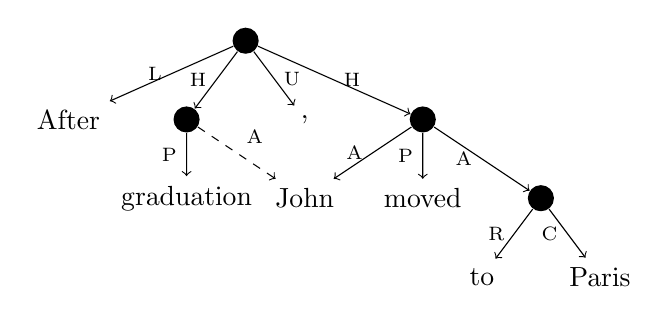
\begin{tikzpicture}[level distance=10mm, ->,
      every circle node/.append style={fill=black}]
    \node (ROOT) [circle] {}
      child {node (After) {After} edge from parent node[left] {\scriptsize L}}
      child {node (graduation) [circle] {}
      {
        child {node {graduation} edge from parent node[left] {\scriptsize P}}
      } edge from parent node[left] {\scriptsize H} }
      child {node {,} edge from parent node[right] {\scriptsize U}}
      child {node (moved) [circle] {}
      {
        child {node (John) {John} edge from parent node[left] {\scriptsize A}}
        child {node {moved} edge from parent node[left] {\scriptsize P}}
        child {node [circle] {}
        {
          child {node {to} edge from parent node[left] {\scriptsize R}}
          child {node {Paris} edge from parent node[left] {\scriptsize C}}
        } edge from parent node[left] {\scriptsize A} }
      } edge from parent node[right] {\scriptsize H} }
      ;
    \draw[dashed,->] (graduation) to node [auto] {\scriptsize A} (John);
  \end{tikzpicture}
  }}
  \end{subfigure}
  \begin{subfigure}{.9\columnwidth}
  \parbox{.05\columnwidth}{\caption{}\label{fig:gave}}
  \parbox{.75\columnwidth}{\hspace{1cm}
  \scalebox{.9}{
  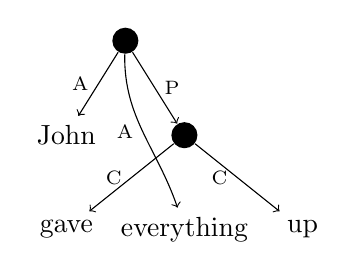
\begin{tikzpicture}[level distance=12mm, ->,
      every node/.append style={midway},
      every circle node/.append style={fill=black}]
    \node (ROOT) [circle] {}
      child {node {John} edge from parent node[left] {\scriptsize A}}
      child {node [circle] {}
      {
      	child {node {gave} edge from parent node[left] {\scriptsize C}}
      	child {node (everything) {everything} edge from parent[white]}
      	child {node {up} edge from parent node[left] {\scriptsize C}}
      } edge from parent node[right] {\scriptsize P} }
      ;
    \draw[bend right,->] (ROOT) to[out=-20, in=180] node [left] {\scriptsize A} (everything);
  \end{tikzpicture}
  }}
  \end{subfigure}
  \begin{subfigure}{.9\columnwidth}
  \parbox{.05\columnwidth}{\caption{}\label{fig:home}}
  \parbox{.65\columnwidth}{
  \scalebox{.9}{
  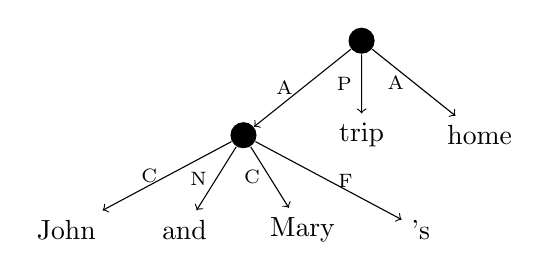
\begin{tikzpicture}[level distance=12mm, ->,
      every node/.append style={midway},
      every circle node/.append style={fill=black}]
    \node (ROOT) [circle] {}
      child {node [circle] {}
      {
        child {node {John} edge from parent node[left] {\scriptsize C}}
        child {node {and} edge from parent node[left] {\scriptsize N}}
        child {node {Mary} edge from parent node[left] {\scriptsize C}}
        child {node {'s} edge from parent node[right] {\scriptsize F}}
      } edge from parent node[left] {\scriptsize A} }
      child {node {trip} edge from parent node[left] {\scriptsize P}}
      child {node {home} edge from parent node[left] {\scriptsize A}}
      ;
  \end{tikzpicture}
  }}
  \end{subfigure}
  \caption{\label{fig:examples}
    UCCA structures demonstrating three structural properties exhibited by
    the scheme.
    (\subref{fig:graduation}) includes a remote edge (dashed),
    resulting in ``John'' having two parents.
    (\subref{fig:gave}) includes a discontinuous unit (``gave ... up'').
    (\subref{fig:home}) includes a coordination construction (``John and Mary'').
    Pre-terminal nodes are omitted for brevity.
  }
\end{figure}

\paragraph{Coverage.}
The \textit{coverage} $\mathcal{C}$ of a transition system coupled with an oracle is the set of graphs
it can assign to any input $\langle w\rangle_1^n$ \cite{kuhlmann2010transition}.
A system with coverage $\mathcal{C}$ is \textit{complete} with respect to a set of graphs $mathcal{G}$
if $\mathcal{G}\subseteq\mathcal{C}$, and \textit{sound} with respect to it if
$\mathcal{C}\subseteq\mathcal{G}$.

We present a general transition system for graph parsing,
and show both by means of a formal proof and by experimental means that
it is complete and sound with respect to the class of anchored graphs $\mathcal{A}$.\footnote{Our
code will be made freely available upon publication.}

The rest of the paper is structured as follows:
\secref{sec:system} describes our transition system.
\secref{sec:completeness} proves our transition system is complete with respect to anchored graphs, and
\secref{sec:soundness} proves it is sound.
\secref{sec:related_work} summarizes related work, and
\secref{sec:conclusion} concludes the paper.


%%%%%%%%%%%%%%%%%%%%%%%%%%%%%%%%%%%%%%%%%%%%%%%%%%%%%%%%%%%%%%%
\section{Transition System}\label{sec:system}

Given a sequence of tokens $w_1, \ldots, w_n$, we predict a graph $G$ over the sequence.
Parsing starts with a single node on the stack (an artificial root node), and the input tokens
in the buffer. \figref{fig:transitions} shows the transition set.

\paragraph{Transition set.}
In addition to the standard \textsc{Shift} and \textsc{Reduce} operations, 
we follow previous work in transition-based constituency parsing \cite{sagae2005classifier},
adding the \textsc{Node} transition for creating new non-terminal nodes.
For every $X\in L$,
\textsc{Node$_X$} creates a new node on the buffer as a parent of the first element on the stack, with an $X$-labeled edge.

\textsc{Implicit$_X$} acts similarly, but the created node is a child instead,
representing a unit that does not appear explicitly in the text.

\textsc{Left-Edge$_X$} and \textsc{Right-Edge$_X$} create a new primary $X$-labeled edge
between the first two elements on the stack,
where the parent is the left or the right node, respectively.
To support the prediction of multiple parents, node and edge transitions
leave the stack unchanged, as in other work on
transition-based dependency graph parsing
\cite{sagae2008shift,ribeyre-villemontedelaclergerie-seddah:2014:SemEval,tokgoz2015transition}.

\textsc{Reduce} pops the stack, to allow removing a node
once all its edges have been created.

To handle discontinuous nodes, \textsc{Swap} pops the second
node on the stack and adds it to the top of the buffer, as with the similarly
named transition in previous work \cite{nivre2009non,maier2015discontinuous}.
This transition uses the notion of a \textit{swap index}:
intuitively, this index reflects the "natural order" of nodes,
according to the order of terminals in the text and the terminal descendants of non-terminal nodes.
The root's swap index is 0, and for each terminal, its swap index is its position in the text
(starting for 1 for the first terminal).
Whenever a non-terminal node is created, its swap index is the arithmetic mean between
the swap indices of the top of the stack ($s_0$) and the first element in the buffer ($b_0$).
This is appropriate, since for any node-creating transition, the new node is created
as the first element on the buffer, i.e., in between $s_0$ and the current $b_0$.


Finally, \textsc{Finish} pops the root node and marks the state as terminal.

\begin{figure*}
	\begin{adjustbox}{width=\textwidth,margin=3pt,frame}
	\begin{tabular}{llll|l|llllc|c}
		\multicolumn{4}{c|}{\textbf{\small Before Transition}} & \textbf{\small Transition} & \multicolumn{5}{c|}{\textbf{\small After Transition}} & \textbf{\small Condition} \\
		\textbf{\footnotesize Stack} & \textbf{\footnotesize Buffer} & \textbf{\footnotesize Nodes} & \textbf{\footnotesize Edges} & & \textbf{\footnotesize Stack} & \textbf{\footnotesize Buffer} & \textbf{\footnotesize Nodes} & \textbf{\footnotesize Edges} & \textbf{\footnotesize Terminal?} & \\
		$S$ & $x \;|\; B$ & $V$ & $E$ & \textsc{Shift} & $S \;|\; x$ & $B$ & $V$ & $E$ & $-$ & \\
		$S \;|\; x$ & $B$ & $V$ & $E$ & \textsc{Reduce} & $S$ & $B$ & $V$ & $E$ & $-$ & \\
		$S \;|\; x$ & $B$ & $V$ & $E$ & \textsc{Node$_X$} & $S \;|\; x$ & $y \;|\; B$ & $V \cup \{ y \}$ & $E \cup \{ (y,x)_X \}$ & $-$ &
		$x \neq \mathrm{root}$ \\
		$S \;|\; x$ & $B$ & $V$ & $E$ & \textsc{Implicit$_X$} & $S \;|\; x$ & $y^* \;|\; B$ & $V \cup \{ y^* \}$ & $E \cup \{ (x,y^*)_X \}$ & $-$ & $x \not\in w_{1:n}$ \\
		$S \;|\; y,x$ & $B$ & $V$ & $E$ & \textsc{Left-Edge$_X$} & $S \;|\; y,x$ & $B$ & $V$ & $E \cup \{ (x,y)_X \}$ & $-$ &
		\multirow{4}{50pt}{\vspace{-1cm}\[\left\{\begin{array}{l}
		x \not\in w_{1:n},\\
		y \neq \mathrm{root}
		\end{array}\right.\]} \\
		$S \;|\; x,y$ & $B$ & $V$ & $E$ & \textsc{Right-Edge$_X$} & $S \;|\; x,y$ & $B$ & $V$ & $E \cup \{ (x,y)_X \}$ & $-$ & \\
		$S \;|\; x,y$ & $B$ & $V$ & $E$ & \textsc{Swap} & $S \;|\; y$ & $x \;|\; B$ & $V$ & $E$ & $-$ &
		$\mathrm{i}(x) < \mathrm{i}(y)$ \\
		$[\mathrm{root}]$ & $\emptyset$ & $V$ & $E$ & \textsc{Finish} & $\emptyset$ & $\emptyset$ & $V$ & $E$ & $+$ & \\
	\end{tabular}
	\end{adjustbox}
	\caption{\label{fig:transitions}
	  Transition set for graph parsing.
	  We write the stack with its top to the right and the buffer with its head to the left.
	  $(\cdot,\cdot)_X$ denotes an $X$-labeled edge.
	  $\mathrm{i}(x)$ is the swap index of node $x$.
	}
\end{figure*}

\paragraph{Oracle.}
For training a transition-based parser, we can use an \textit{oracle}.
In general, it is better to use a \textit{dynamic oracle} \cite{goldberg2012dynamic},
i.e., an oracle that outputs a set of optimal transitions: when
applied to the current parser state, the gold
standard graph is reachable from the resulting state.
Another sense of \textit{dynamic oracle} refers to \textit{training with exploration}
\cite{goldberg2013dynamic,goldberg2013training,ballesteros-EtAl:2016:EMNLP2016}:
rather than maintaining a state where the gold standard graph is reachable,
the oracle may return a set of optimal transitions at any state,
even if the gold standard graph is not reachable from it.

In our case, the oracle would predict a \textsc{Node} transition if the stack 
has on its top a parent in the gold graph that has not been created,
but would predict a \textsc{Right-Edge} transition if the second stack
element is a parent of the
first element according to the gold graph and the edge between them has not been created.
The transition predicted by the classifier is deemed correct
and is applied to the parser state to reach the subsequent state,
if the transition is included in the set of optimal transitions.
Otherwise, a random optimal transition is applied,
and for the perceptron-based parser, the classifier's weights are updated according
to the perceptron update rule.


%%%%%%%%%%%%%%%%%%%%%%%%%%%%%%%%%%%%%%%%%%%%%%%%%%%%%%%%%%%%%%%
\section{Completeness}\label{sec:completeness}

Here we sketch a proof for the fact that the transition set defined in \cite{hershcovich2017a}
is capable of producing any rooted, labeled, anchored graph.
This proves that the transition set is complete with respect to anchored graphs.

Let $G=(V,E,\ell)$ be a graph with labels $\ell:E\rightarrow L$
over a sequence of tokens $w_1, \ldots, w_n$.
Parsing starts with $w_1, \ldots, w_n$ on the buffer,
and the root node on the stack.

First we show that every node can be created, by induction on the node height:
every terminal (height zero) already exists at the beginning of the parse
(and so does the root node).
Let $v\in V$ be of height $k$, and assume all nodes of height less than $k$ can be created.
Take any (primary) child $u$ of $v$: its height must be less than $k$.
If $u$ is a terminal, apply \textsc{Shift} until it lies at the head of the buffer.
Otherwise, by our assumption, $u$ can still be created.
Right after $u$ is created, it lies at the head of the buffer.
A \textsc{Shift} transition followed by a \textsc{Node}$_{\ell(v,u)}$ transition will
move $u$ to the stack and create $v$ on the buffer, with the correct edge label.

Next, we show that every edge can be created.
Let $(v,u) \in E$ be any edge with parent $v$ and child $u$.
Assume $v$ and $u$ have both been created (we already showed that both are created eventually).
If either $v$ or $u$ are in the buffer, apply \textsc{Shift} until both are in the stack.
If both are in the stack but neither is at the stack top, apply \textsc{Swap} transitions
until either moves to the buffer, and then apply \textsc{Shift}.
Now, assume either $v$ or $u$ is at the stack top.
If the other is not the second element on the stack, apply \textsc{Swap} transitions until it is.
Finally, $v$ and $u$ are the top two elements on the stack.
If they are in that order, apply \textsc{Right-Edge}$_{\ell(v,u)}$
(or \textsc{Right-Remote}$_{\ell(v,u)}$ if the edge between them is remote).
Otherwise, apply \textsc{Left-Edge}$_{\ell(v,u)}$
(or \textsc{Left-Remote}$_{\ell(v,u)}$ if the edge between them is remote).
This creates $(v,u)$ with the correct edge label.

Once all nodes and edges have been created, we can apply \textsc{Reduce} until only the
root node remains on the stack, and then \textsc{Finish}.
This yields exactly the graph $G$.


%%%%%%%%%%%%%%%%%%%%%%%%%%%%%%%%%%%%%%%%%%%%%%%%%%%%%%%%%%%%%%%
\section{Soundness}\label{sec:soundness}

We now turn to prove the fact that every transition sequence allowed by our transition system
indeed corresponds to a valid anchored graph.


%%%%%%%%%%%%%%%%%%%%%%%%%%%%%%%%%%%%%%%%%%%%%%%%%%%%%%%%%%%%%%%

\section{Related Work}\label{sec:related_work}



%%%%%%%%%%%%%%%%%%%%%%%%%%%%%%%%%%%%%%%%%%%%%%%%%%%%%%%%%%%%%%%
\section{Conclusion}\label{sec:conclusion}



%%%%%%%%%%%%%%%%%%%%%%%%%%%%%%%%%%%%%%%%%%%%%%%%%%%%%%%%%%%%%%%
%\section*{Acknowledgments}
%
%This work was supported by the HUJI Cyber Security Research Center
%in conjunction with the Israel National Cyber Bureau in the Prime Minister's Office,
%and by the Intel Collaborative Research Institute for Computational Intelligence (ICRI-CI).
%The first author was supported by a fellowship from the
%Edmond and Lily Safra Center for Brain Sciences.
%We thank Wolfgang Maier, Nathan Schneider, Elior Sulem
%and the anonymous reviewers for their helpful comments.


\bibliography{references}
\bibliographystyle{acl_natbib}

\end{document}

